%----------------------------------------------------------------------------------------
%	PACKAGES AND THEMES
%----------------------------------------------------------------------------------------


\documentclass{beamer}

\mode<presentation> {

% The Beamer class comes with a number of default slide themes
% which change the colors and layouts of slides. Below this is a list
% of all the themes, uncomment each in turn to see what they look like.


\usepackage{qtree}
\usepackage{amsthm}
\usepackage{algpseudocode}
\usepackage[export]{adjustbox}
\usepackage{subcaption}
\usepackage{hyperref}
\usepackage{graphicx}
\usepackage{tabularx}
\usepackage{mdframed}
\usepackage{framed}
\usepackage{siunitx}
\usepackage{placeins}
\usepackage{units}
\usepackage{xcolor}
\usepackage{lipsum}
\usepackage{algorithm}
\usepackage{amsmath}
\usepackage{paralist}
\usepackage{mdwlist}
\usepackage[labeled]{multibib}
\usepackage{array}
\usepackage{newfloat}
\usepackage{datetime}

%\usetheme{default}
%\usetheme{AnnArbor}
%\usetheme{Antibes}
%\usetheme{Bergen}
%\usetheme{Berkeley}
%\usetheme{Berlin}
%\usetheme{Boadilla}
%\usetheme{CambridgeUS}
%\usetheme{Copenhagen}
%\usetheme{Darmstadt}
%\usetheme{Dresden}
%\usetheme{Frankfurt}
%\usetheme{Goettingen}
%\usetheme{Hannover}
%\usetheme{Ilmenau}
%\usetheme{JuanLesPins}

%\usetheme{Luebeck}
\usetheme{Madrid}
%\usetheme{Malmoe}
%\usetheme{Marburg}
%\usetheme{Montpellier}
%\usetheme{PaloAlto}
%\usetheme{Pittsburgh}
%\usetheme{Rochester}
%\usetheme{Singapore}
%\usetheme{Szeged}
%\usetheme{Warsaw}

% As well as themes, the Beamer class has a number of color themes
% for any slide theme. Uncomment each of these in turn to see how it
% changes the colors of your current slide theme.

%\usecolortheme{albatross}
%\usecolortheme{beaver}
%\usecolortheme{beetle}
%\usecolortheme{crane}
%\usecolortheme{dolphin}
%\usecolortheme{dove}
%\usecolortheme{fly}
%\usecolortheme{lily}
%\usecolortheme{orchid}
%\usecolortheme{rose}
%\usecolortheme{seagull}
%\usecolortheme{seahorse}
%\usecolortheme{whale}
%\usecolortheme{wolverine}

%\setbeamertemplate{footline} % To remove the footer line in all slides uncomment this line
%\setbeamertemplate{footline}[page number] % To replace the footer line in all slides with a simple slide count uncomment this line

%\setbeamertemplate{navigation symbols}{} % To remove the navigation symbols from the bottom of all slides uncomment this line
}

\usepackage{graphicx} % Allows including images
\usepackage{booktabs} % Allows the use of \toprule, \midrule and \bottomrule in tables

%----------------------------------------------------------------------------------------
%	TITLE PAGE
%----------------------------------------------------------------------------------------

\title[Wavelet Tree]{Engineering Rank and Select Queries on Wavelet Trees} % The short title appears at the bottom of every slide, the full title is only on the title page

\author{Roland Larsen Pedersen} % Your name
\institute[Datalogi] % Your institution as it will appear on the bottom of every slide, may be shorthand to save space
{
Datalogi, Aarhus Universitet \\ % Your institution for the title page
\medskip
\textit{Thesis defence}
}
\date{June 25, 2015} % Date, can be changed to a custom date

\begin{document}

\begin{frame}
\titlepage % Print the title page as the first slide
\end{frame}

\begin{frame}
\frametitle{Overview} % Table of contents slide, comment this block out to remove it
\tableofcontents % Throughout your presentation, if you choose to use \section{} and \subsection{} commands, these will automatically be printed on this slide as an overview of your presentation
\end{frame}

%----------------------------------------------------------------------------------------
%	PRESENTATION SLIDES
%----------------------------------------------------------------------------------------


\section{What is a Wavelet Tree?}

\subsection{Definitions}
\begin{frame}
\frametitle{Wavelet Tree: Definitions}
\begin{itemize}
\item In its basic form, the wavelet tree is a balanced binary tree. 
\item It stores a \textit{sequence} $S[1,n] = c_1c_2c_3 \ldots c_n$ of \textit{symbols} $c_i \in \Sigma$, where $\Sigma = [1 \ldots \sigma]$ is the \textit{alphabet} of $S$.
\item The tree has height $h = \lceil \log \sigma \rceil$, and $2 \sigma - 1$ nodes, with $\sigma$ of those as leaf nodes and $\sigma - 1$ as internal nodes.
\end{itemize}

\end{frame}


%------------------------------------------------

\begin{frame}
\frametitle{Constructing the Wavelet Tree}
\begin{itemize}
\item The wavelet tree is constructed recursively, starting at the root node and moving down the tree, with each node in the tree receiving a string constructed by its parent, except the root node that receives the full input string.
\item Each node calculates the middle character of $\Sigma$ and uses it to set the bits in the bitmap and split $S$ in two substrings $S_{\mathit{left}}$ and $S_{\mathit{right}}$.
\end{itemize}
\end{frame}

%------------------------------------------------
\subsection{Constructing the Wavelet Tree}
\begin{frame}
\frametitle{Wavelet Tree Example}
\Tree
%root
[.adsfadaadsfaads\\001100000110001 !\qsetw{5cm} 
	%left child
	[.adadaadaad\\0101001001 !\qsetw{5cm}
		%left -> left,right child 
		[.aaaaaa !\qsetw{5cm} ] [.dddd !\qsetw{5cm} ]] 
	%right child
	[.sfsfs\\10101 !\qsetw{5cm} 
		%right -> left,right child
		[.ff !\qsetw{5.3cm} ] [.sss !\qsetw{5.3cm} ]]] 
\vspace*{1cm}		
$S = \text{adsfadaadsfaads}, \Sigma = \text{adfs}$
\end{frame}

%------------------------------------------------
\begin{frame}
\frametitle{Construction time and memory usage}
\begin{itemize}
\item Construction time: $O(n \cdot h) = O(n \log \sigma)$
	\begin{itemize}
	\item The Wavelet Tree can theoretically be constructed in $O(n \cdot h) = O(n \log \sigma)$ time as the sum of the lengths of the strings being processed at any single layer of the tree is the length of the input string to the tree.
	\end{itemize}
\item Memory usage: $O(n \log \sigma + \sigma \cdot \mathit{ws})$ bits
	\begin{itemize}
	\item At each level in the tree at most \textit{n} bits are stored in the bitmaps in total, making $n \cdot h = n \cdot \log \sigma$ an upper bound to the total number of bits that a wavelet tree stores in its bitmaps.
\item In addition to this, each node takes some constant amount of machine words of space, and there are $2 \sigma -1$ nodes in the tree.
\textit{ws} is the size of our machine words.
This makes the total memory consumption $O(n \log \sigma + \sigma \cdot \mathit{ws})$ bits.
	\end{itemize}
\end{itemize}
\end{frame}

\section{Queries}
%------------------------------------------------
\begin{frame}
\frametitle{Wavelet Tree: Queries}
\begin{itemize}
\item The wavelet tree supports three queries:
	\begin{itemize}
	\item \textbf{Access(p)}: Return the character \textit{c} at position \textit{p} in sequence \textit{S}.
		\begin{itemize}
		\item Running time: $O(n \log \sigma)$.
		\item We have not implemented Access because it resembles Rank.
		\end{itemize}
	\item \textbf{Rank(c, p)}: Return the number of occurrences of character \textit{c} in \textit{S} up to position \textit{p}.
		\begin{itemize}
		\item Running time: $O(n \log \sigma)$.
		\end{itemize}
	\item \textbf{Select(c, o)}: Return the position of the \textit{o}th occurrence of character \textit{c} in \textit{S}.
		\begin{itemize}
		\item Running time: $O(n \log \sigma)$
		\end{itemize}
	\end{itemize}
\end{itemize}

\end{frame}

%------------------------------------------------

\subsection{Rank}
\begin{frame}
\frametitle{Rank on a Wavelet Tree}
\begin{center}
	\center 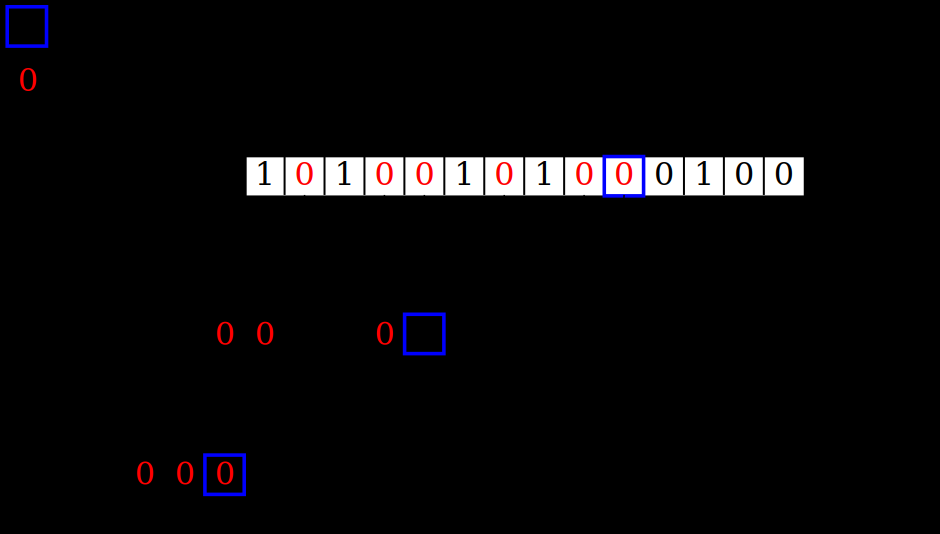
\includegraphics[width=0.8\textwidth]{RankDrawing}
\end{center}
\end{frame}

%------------------------------------------------

\subsection{Select}
\begin{frame}
\frametitle{Select on a Wavelet Tree}
\begin{center}
	\includegraphics[width=0.8\textwidth]{SelectDrawing}
\end{center}
\end{frame}

\section{Applications}
%------------------------------------------------
\begin{frame}
\frametitle{Wavelet Tree: Applications}
\begin{itemize}
\item Compression
	\begin{itemize}
	\item Zero-order entropy compression ($H_0$) using a RLE Wavelet Tree or a Huffman Shaped Wavelet Tree.
	\item Higher-order entropy compression ($H_k$) using Burrows-Wheeler transformation and a RLE wavelet tree.
	\item $H_k <= H_0 <= \log \sigma$.
	\end{itemize}
\item Information Retrieval
	\begin{itemize}
	\item Positional inverted index
	\item Document retrieval
	\item Range Quantile Query: Return the \textit{k}th smallest number within a subsequence of a given sequence of elements.
	\item FM-count: Return number of occurrences of a pattern p in S. 
	\end{itemize}
\end{itemize}
\end{frame}

\subsection{Compression}
%------------------------------------------------
\subsubsection{Run-length encoding}
\begin{frame}
\frametitle{Compression: Run-length encoding}
\begin{itemize}
\item Run-length encoding counts the number of consecutive occurrences of a symbol and substitutes the consecutive occurrences with the symbol followed by its number of occurrences.
\item Example: $RLE(\text{aaaaabbbaacccccaaaaa}) = \text{a5,b3,a2,c5,a5}$.
\item Binary example: $RLE(00000000001111100000) = 10,5,5 $
	\begin{itemize}
	\item We can avoid specifying the symbol by assuming that $0$ is always the first symbol.
	\item If the binary number begins with a $1$ we just add a $0$ to the beginning of the result.
	\end{itemize}
\item Query by reversing RLE. It takes linear time $O(n)$ to reverse. Rank and select query time becomes $O(2n \log \sigma) = O(n \log \sigma)$
\item Achieves space complexity within $H_0$
\end{itemize}
\end{frame}


%------------------------------------------------
\begin{frame}
\frametitle{RLE Wavelet Tree on string \textit{bananahat} with alphabet $\Sigma =$ \textit{abhnt}}
\begin{figure}
\begin{subfigure}{0.49\textwidth}     
\Tree
%root
[.bananahat\\001010001 !\qsetw{3cm} 
	%left child
	[.baaaha\\000011 !\qsetw{3cm}
		[.baaaa\\10000 !\qsetw{3cm}
			[.aaaa !\qsetw{3cm} ]
			[.b !\qsetw{3cm} ]		
		] 
		[.h !\qsetw{3cm} ]
	] 
	%right child
	[.nnt\\001 !\qsetw{3cm}	
		[.nn !\qsetw{3cm} ] 
		[.t !\qsetw{3cm} ]
	]
]
		\caption{Wavelet Tree on string \textit{bananahat} with alphabet $\Sigma =$ \textit{abhnt}}
\end{subfigure}
\hfill
\begin{subfigure}{0.49\textwidth}	
\Tree
%root
[.bananahat\\2,1,1,1,3,1 !\qsetw{3cm} 
	%left child
	[.baaaha\\4,1,1 !\qsetw{3cm}
		[.baaaa\\0,1,4 !\qsetw{3cm}
			[.aaaa !\qsetw{3cm} ]
			[.b !\qsetw{3cm} ]		
		] 
		[.h !\qsetw{3cm} ]
	] 
	%right child
	[.nnt\\2,1 !\qsetw{3cm}	
		[.nn !\qsetw{3cm} ] 
		[.t !\qsetw{3cm} ]
	]
]
\caption{RLE Wavelet Tree on string \textit{bananahat} with alphabet $\Sigma =$ \textit{abhnt}}
\end{subfigure}
\end{figure}
\end{frame}


\subsubsection{Burrows-Wheeler Transform}
%------------------------------------------------
\begin{frame}
\frametitle{Compression: Burrows-Wheeler transform}
\begin{itemize}
\item BWT permutes the order of the characters. If the original string had several substrings that occurred often, then the transformed string will have several places where a single character is repeated multiple times in a row.
\item As a result it groups symbols more which improves the effect of Run-length encoding
\item BWT is reversible
\item Combined with RLE Wavelet Tree it achieves $H_k$ compression.
\end{itemize}
\end{frame}

\begin{frame}
\frametitle{BWT example}
$S = $ bananahat.
\begin{center}
$\begin{bmatrix}
	bananahat\#\\
	ananahat\#b\\
	nanahat\#ba\\
	anahat\#ban\\
	nahat\#bana\\
	ahat\#banan\\
	hat\#banana\\
	at\#bananah\\
	t\#bananaha\\
	\#bananahat\\
\end{bmatrix} \Rightarrow
\begin{bmatrix}
	\#bananaha\textbf{t}\\
	ahat\#bana\textbf{n}\\
	anahat\#ba\textbf{n}\\
	ananahat\#\textbf{b}\\
	at\#banana\textbf{h}\\
	bananahat\#\\
	hat\#banan\textbf{a}\\
	nahat\#ban\textbf{a}\\
	nanahat\#b\textbf{a}\\
	t\#bananah\textbf{a}
\end{bmatrix}$
\end{center}
$BWT(S) = $ tnnbhaaaa.
\end{frame}

%------------------------------------------------
\begin{frame}
\frametitle{Burrows-Wheeler reverse transform example}
$S = \text{dca}$
\begin{center}
$M = \begin{bmatrix}
	dca\#\\
	ca\#d\\
	a\#dc\\
	\#dca
\end{bmatrix} \Rightarrow
M' = 
\begin{bmatrix}
	\#dc\textbf{a}\\
	a\#d\textbf{c}\\
	ca\#\textbf{d}\\
	dca\textbf{\#}
\end{bmatrix}$\\
\end{center}
$BWT(S) = acd$
\vspace{0.5cm}

Reverse BWT:
\begin{tabular}{|l|l|l|l|l|l|l|l|}
\hline
Add 1 & Sort 1 & Add 2 & Sort 2 & Add 3 & Sort 3 & Add 4 & Sort 4\\
\hline 
\begin{tabular}{@{}>{$}l<{$}@{}}
	a\\ c\\ d\\ \#
\end{tabular} & 
\begin{tabular}{@{}>{$}l<{$}@{}}
	\#\\ a\\ c\\ d
\end{tabular} & 
\begin{tabular}{@{}>{$}l<{$}@{}}
	a\#\\ ca\\ dc\\ \#d
\end{tabular} & 
\begin{tabular}{@{}>{$}l<{$}@{}}
	\#d\\ a\#\\ ca\\ dc
\end{tabular} & 
\begin{tabular}{@{}>{$}l<{$}@{}}
	a\#d\\ ca\#\\ dca\\ \#dc
\end{tabular} & 
\begin{tabular}{@{}>{$}l<{$}@{}}
	\#dc\\ a\#d\\ ca\#\\ dca
\end{tabular} & 
\begin{tabular}{@{}>{$}l<{$}@{}}
	a\#dc\\ ca\#d\\ dca\#\\ \#dca
\end{tabular} &
\begin{tabular}{@{}>{$}l<{$}@{}}
	\#dca\\ a\#dc\\ ca\#d\\ \textbf{dca\#}\\
\end{tabular} \\ \hline
\end{tabular}
*$\# = \text{end of line character}$
\end{frame}

%----------------------------------------------------------------------------------------
\begin{frame}
\frametitle{RLE Wavelet Tree on string \textit{bananahat} with alphabet $\Sigma =$ \textit{abhnt}}
\begin{figure}
\begin{subfigure}{0.49\textwidth}     
\Tree
%root
[.bananahat\\2,1,1,1,3,1 !\qsetw{3cm} 
	%left child
	[.baaaha\\4,1,1 !\qsetw{3cm}
		[.baaaa\\0,1,4 !\qsetw{3cm}
			[.aaaa !\qsetw{3cm} ]
			[.b !\qsetw{3cm} ]		
		] 
		[.h !\qsetw{3cm} ]
	] 
	%right child
	[.nnt\\2,1 !\qsetw{3cm}	
		[.nn !\qsetw{3cm} ] 
		[.t !\qsetw{3cm} ]
	]
]
\caption{RLE Wavelet Tree on string \textit{bananahat} with alphabet $\Sigma =$ \textit{abhnt}}
\end{subfigure}
\hfill
\begin{subfigure}{0.49\textwidth}	
\Tree
%root
[.tnnbhaaaa\\\textbf{0,3,6} !\qsetw{3cm} 
	%left child
	[.bhaaaa\\1,1,4 !\qsetw{3cm} 
		[.baaaa\\0,1,4 !\qsetw{3cm} 
			[.aaaa !\qsetw{3cm} ]
			[.b !\qsetw{3cm} ]		
		] 
		[.h !\qsetw{3cm} ]
	] 
	%right child
	[.tnn\\0,1,2 !\qsetw{3cm}		
		[.nn !\qsetw{3cm} ] 
		[.t !\qsetw{3cm} ]
	]
]
\caption{BWT RLE Wavelet Tree on string \textit{tnnbhaaaa} with alphabet $\Sigma =$ \textit{abhnt}}
\end{subfigure}
\end{figure}
\end{frame}

\subsubsection{Huffman Shaped Wavelet tree}
%----------------------------------------------------------------------------------------
\begin{frame}
\frametitle{Huffman shaped wavelet tree}
\begin{itemize}
\item Use Huffman codes of symbols to shape the tree
\item A Huffman code is a binary value assigned to each symbol. The symbol with the highest frequency gets the lowest value.
\item Shaping the tree based on Huffman codes places the most frequent symbols at the top of the tree and least frequent symbols at the bottom of the tree.
\item Huffman shaping only makes sense on non-uniformly distributed data like a natural language text.

\end{itemize}
\end{frame}

%----------------------------------------------------------------------------------------
\begin{frame}
\frametitle{Huffman Shaped Wavelet Tree: Example}
\hspace*{2cm}Wavelet Tree: \hspace{3cm} Huffman Shaped WT:
\begin{center}
	\center 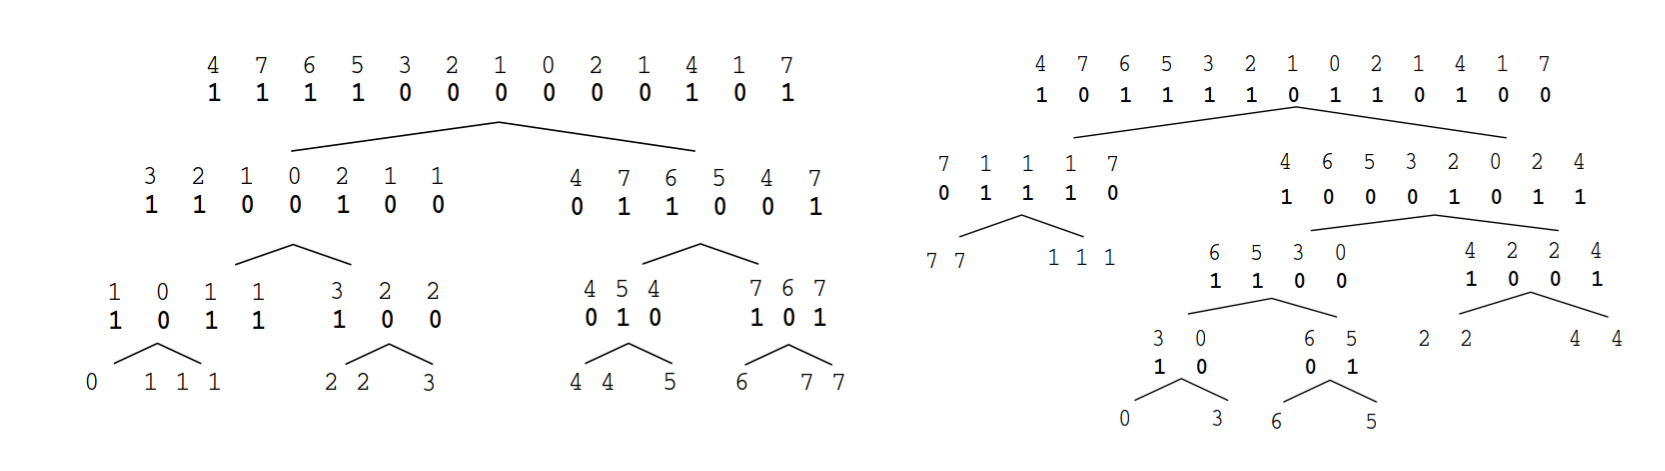
\includegraphics[width=1.0\textwidth]{Huffman-shaped-wavelet-tree}
\end{center}
\end{frame}

%----------------------------------------------------------------------------------------
\begin{frame}
\frametitle{Huffman Shaped WT: Space complexity}
\begin{itemize}
\item Balanced version: $n \log \sigma + o(n \log\sigma) + O(\sigma \log n)$ bits
\item Huffman-shaped: $n(H_0(S) + 1) + o(n(H_0(S) + 1)) + O(\sigma \log n)$ bits. [Efficient Compressed Wavelet Trees over Large Alphabets by Navarro et al.]
\item Huffman-shaped + Compressed Bitmap (RLE): $nH_0(S) + o(n(H_0(S) + 1)) + O(\sigma \log n)$ bits.

\end{itemize}
\end{frame}


%----------------------------------------------------------------------------------------
\begin{frame}
\frametitle{Information Retrieval}
\begin{itemize}
\item k
\end{itemize}
\end{frame}

%----------------------------------------------------------------------------------------

\begin{frame}
\Huge{\centerline{The End}}
\end{frame}

%----------------------------------------------------------------------------------------

\end{document} 